% Cloudflare connection (web/): the laptop POSTs each max-cut Result to the Worker with the DEVICE_TOKEN
% bearer token; the Worker checks it and forwards /api/* to the single DeviceSession Durable Object, which
% validates the Result (protocol/messages.ts isResult), stores the latest one and pushes it to every browser
% over a WebSocket. The React app is served as static assets from the same domain.
% Build: lualatex cloudflare.tex && pdftoppm -png -r 300 -singlefile cloudflare.pdf cloudflare
\documentclass[border=8pt]{standalone}
\usepackage{tikz}
\usetikzlibrary{arrows.meta, positioning}
\usepackage{fontspec}
\setmainfont{TeX Gyre Heros}

\begin{document}
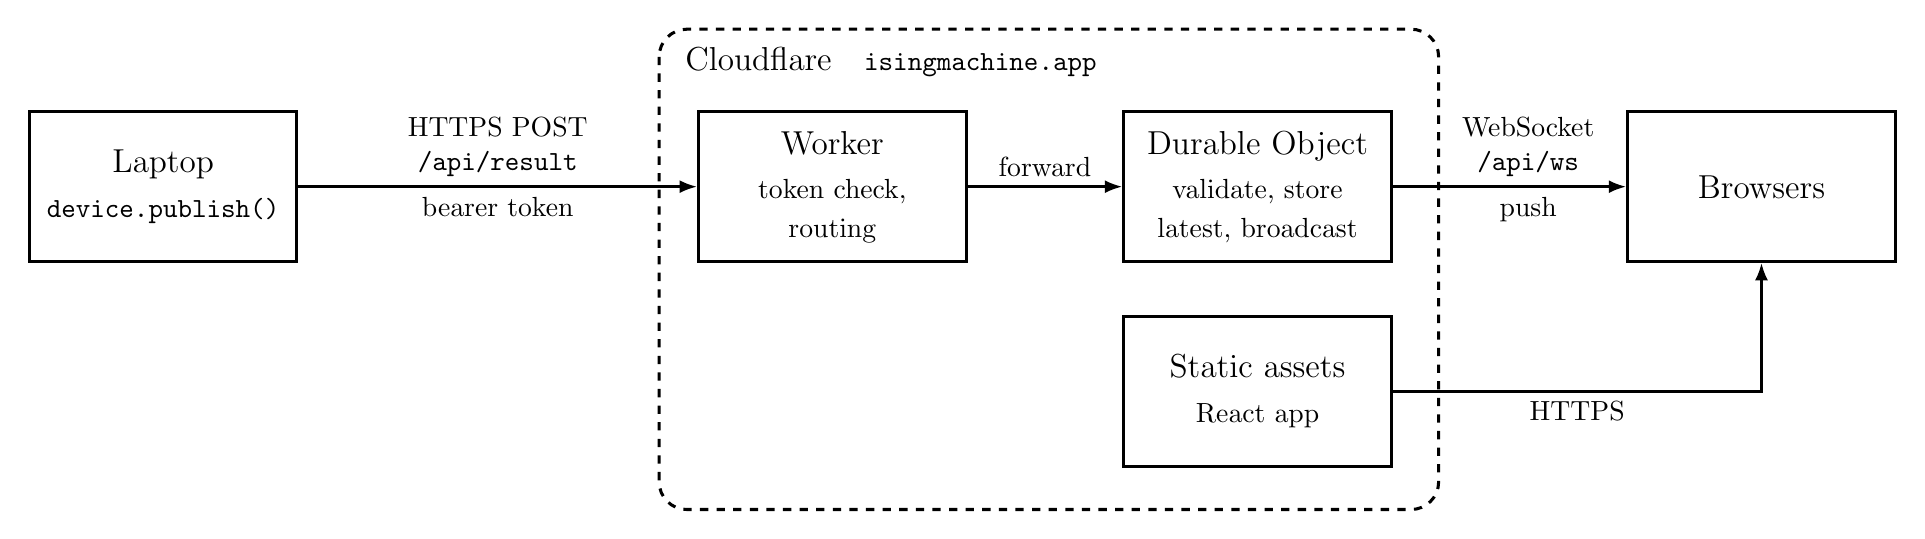
\begin{tikzpicture}[
    font=\large, line width=0.9pt, >={Latex[length=2.2mm]},
    box/.style={draw, line width=1.1pt, align=center, minimum height=1.9cm, minimum width=3.4cm},
    lbl/.style={font=\normalsize},
  ]
  % Cloudflare region
  \draw[line width=1.1pt, dashed, rounded corners=10pt] (4.7,2.0) rectangle (14.6,-4.1);
  \node[anchor=north west] at (4.9,1.9) {Cloudflare\quad\normalsize\texttt{isingmachine.app}};

  % Laptop
  \node[box] (pc) at (-1.6,0) {Laptop\\[2pt]{\normalsize\ttfamily device.publish()}};

  % Worker and Durable Object
  \node[box] (worker) at (6.9,0) {Worker\\[2pt]{\normalsize token check,}\\{\normalsize routing}};
  \node[box] (do) at (12.3,0) {Durable Object\\[2pt]{\normalsize validate, store}\\{\normalsize latest, broadcast}};
  \node[box] (assets) at (12.3,-2.6) {Static assets\\[2pt]{\normalsize React app}};

  \node[box] (web) at (18.7,0) {Browsers};

  % Flows
  \draw[->] (pc.east) -- node[lbl, above, align=center] {HTTPS POST\\\texttt{/api/result}} node[lbl, below] {bearer token} (worker.west);
  \draw[->] (worker.east) -- node[lbl, above] {forward} (do.west);
  \draw[->] (do.east) -- node[lbl, above, align=center, pos=0.58] {WebSocket\\\texttt{/api/ws}} node[lbl, below, pos=0.58] {push} (web.west);
  \draw[->] (assets.east) -| node[lbl, pos=0.25, below] {HTTPS} (web.south);
\end{tikzpicture}
\end{document}
